\chapter{Theoretical Background} \label{ch:theo-back}

This chapter establishes the physical and computational foundations necessary for the reconstruction of EAS at CONDOR. The chapter begins with the properties and astrophysical context of cosmic rays, followed by the phenomenology of atmospheric particle cascades and the principles of ground-based detection. It then describes the CONDOR observatory and the Monte Carlo simulation framework used to generate the training data. Finally, it introduces the deep learning architectures and explainability methods that form the technical core of this thesis.

\section{Cosmic Rays and High-Energy Astrophysics}

The study of cosmic rays sits at the intersection of particle physics, astrophysics, and cosmology. First discovered in 1912 by Victor Hess~\shortcite{hess1912beobachtungen} through a series of balloon ascents that measured increasing ionization rates with altitude, cosmic rays are not electromagnetic radiation but high-energy subatomic particles, primarily bare atomic nuclei, traveling through space at relativistic speeds~\shortcite{longair2011high}. They carry information about some of the most extreme physical environments in the universe, yet the precise mechanisms behind their acceleration remain one of the central open problems in modern astrophysics~\shortcite{blasi2013origin}.

Decades of space-based and balloon-borne measurements have established a precise picture of the composition of cosmic rays at sub-TeV energies. By particle flux, approximately 89\% of primary cosmic rays are protons, roughly 10\% are helium nuclei, and the remaining fraction consists of heavier atomic nuclei up to iron, alongside electrons, positrons, and traces of antimatter~\shortcite{ParticleDataGroup2024}.

Because these primaries are electrically charged, their propagation through the interstellar and intergalactic medium is governed by the Lorentz force, which continuously deflects their trajectories as they pass through irregular galactic magnetic fields. Over astronomical distances, this deflection randomizes their arrival directions at Earth, permanently erasing the geometric line of sight between their production sites and the observer. As a consequence, identifying cosmic ray sources through arrival direction alone is not generally possible, and indirect tracers such as gamma rays and neutrinos become essential tools.

\subsection{The Energy Spectrum}

The energy spectrum of cosmic rays spans more than twelve orders of magnitude and follows a sequence of power laws of the form 
\begin{equation}
  \Phi(E) \propto E^{-\gamma}  
\end{equation}
where $\Phi(E)$ is the differential flux and $\gamma$ is the spectral index. Rather than a single unbroken power law, the spectrum exhibits well-characterized structural breaks that reflect transitions between different source populations, acceleration limits, and propagation regimes. For example, as illustrated in Figure~\ref{fig:crs-spectrum}, precise measurements of this spectrum reveal distinct steepenings and flattenings at specific energy scales — commonly referred to as the \textit{knee}, the \textit{second knee}, and the \textit{ankle} — each associated with changes in the dominant physical processes governing where and how cosmic rays are produced and transported through the Galaxy. Observations of the spectrum and mass composition are therefore fundamental tools for understanding the origin and acceleration mechanisms of high-energy cosmic rays, and they directly motivate the design of observatories sensitive to specific energy windows, such as the sub-TeV range targeted by CONDOR.

\begin{figure}[ht!]
    \centering
    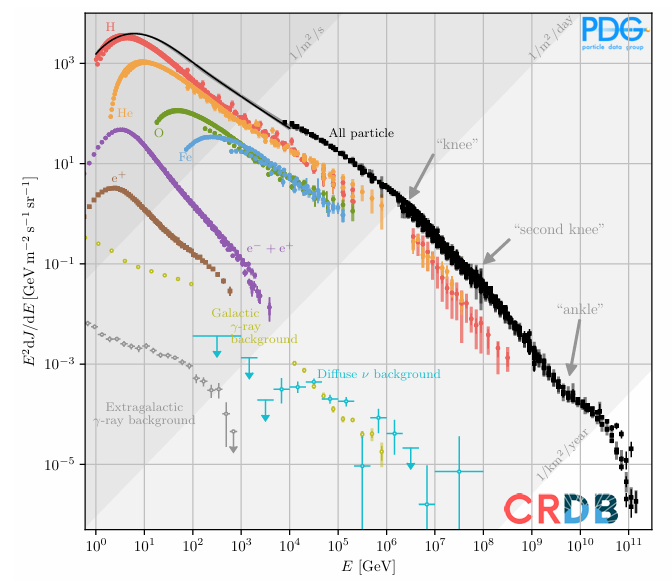
\includegraphics[width=0.65\linewidth]{figures/CRs-energy-spectrum.png}
    \caption[The cosmic ray energy spectrum.]{The cosmic ray energy spectrum. The intensity of charged and neutral cosmic rays, multiplied by kinetic energy squared, is shown as a function of energy. Characteristic breaks such as the knee, second knee, and ankle are clearly visible.}
    \label{fig:crs-spectrum}
\end{figure}

\subsection{Gamma Rays as Cosmic Ray Tracers}

A central motivation for gamma-ray astronomy in the context of cosmic ray physics is that photons, being electrically neutral, are not deflected by interstellar magnetic fields and therefore travel in straight lines from their production sites. This makes them valuable probes of cosmic ray acceleration environments. When a high-energy proton interacts with ambient matter near its source, it produces pions, and neutral pions decay promptly into photon pairs
\begin{equation}
    \pi^0 \to \gamma + \gamma,
\end{equation}
generating gamma-ray emission that directly reflects the parent proton spectrum. Detecting this hadronic signature from a source constitutes direct evidence of cosmic ray acceleration at that site.

However, high-energy electrons can also produce gamma rays through inverse Compton scattering\footnote{Inverse Compton scattering is the process by which a relativistic electron transfers energy to a low-energy photon, up-scattering it to gamma-ray energies; it is the leptonic counterpart to the hadronic $\pi^0$ channel.} and bremsstrahlung\footnote{Bremsstrahlung (German for ``braking radiation'') is the radiation emitted when a charged particle, typically an electron, is deflected by the electric field of an atomic nucleus.}, generating leptonic emission that closely resembles the hadronic signature spectrally. Distinguishing between the two is a central observational challenge, and it is precisely this challenge that motivates the task of gamma-hadron discrimination at ground-based detectors.

\subsection{The Sub-TeV Window}

The energy range between 100 GeV and a few TeV marks the boundary between what is accessible to space-based instruments and what requires ground-based observation. The Fermi-LAT, a space-based pair-conversion gamma-ray telescope 
operating aboard a satellite above the Earth’s atmosphere, effectively detects gamma rays up to a few hundred GeV but is limited by its collection area at higher energies~\shortcite{ackermann2012fermi}. Above this threshold, ground-based detectors exploit the EAS that cosmic rays and gamma rays produce in the atmosphere, reaching the detector level as measurable patterns of secondary particles. CONDOR is designed to operate precisely in this sub-TeV window, and the reconstruction of shower properties in this regime is the central problem addressed in this thesis.

\section{Physics of Extensive Air Showers}

When a high-energy primary particle enters the Earth's atmosphere, it does not reach the ground directly. Instead, its interaction with atmospheric nuclei initiates a cascade of secondary particles that propagates downward at nearly the speed of light, growing in number until the energy per particle drops below the threshold for further multiplication. These cascades, known as extensive air showers, are the fundamental observable that ground-based gamma-ray and cosmic ray observatories exploit~\shortcite{rossi1941cosmic}.

Figure~\ref{fig:cascade_tree} summarizes the sequence of processes that follow the first interaction. The primary produces a large multiplicity of secondary hadrons, mostly pions; the charged ones sustain the hadronic cascade and eventually decay into muons, while the neutral ones decay into photon pairs and transfer their energy into electromagnetic sub-cascades. The three components that reach the ground --- hadronic, muonic and electromagnetic --- are what a surface array actually samples, and the following subsections describe the electromagnetic and hadronic branches in turn.

\begin{figure}[ht!]
    \centering
    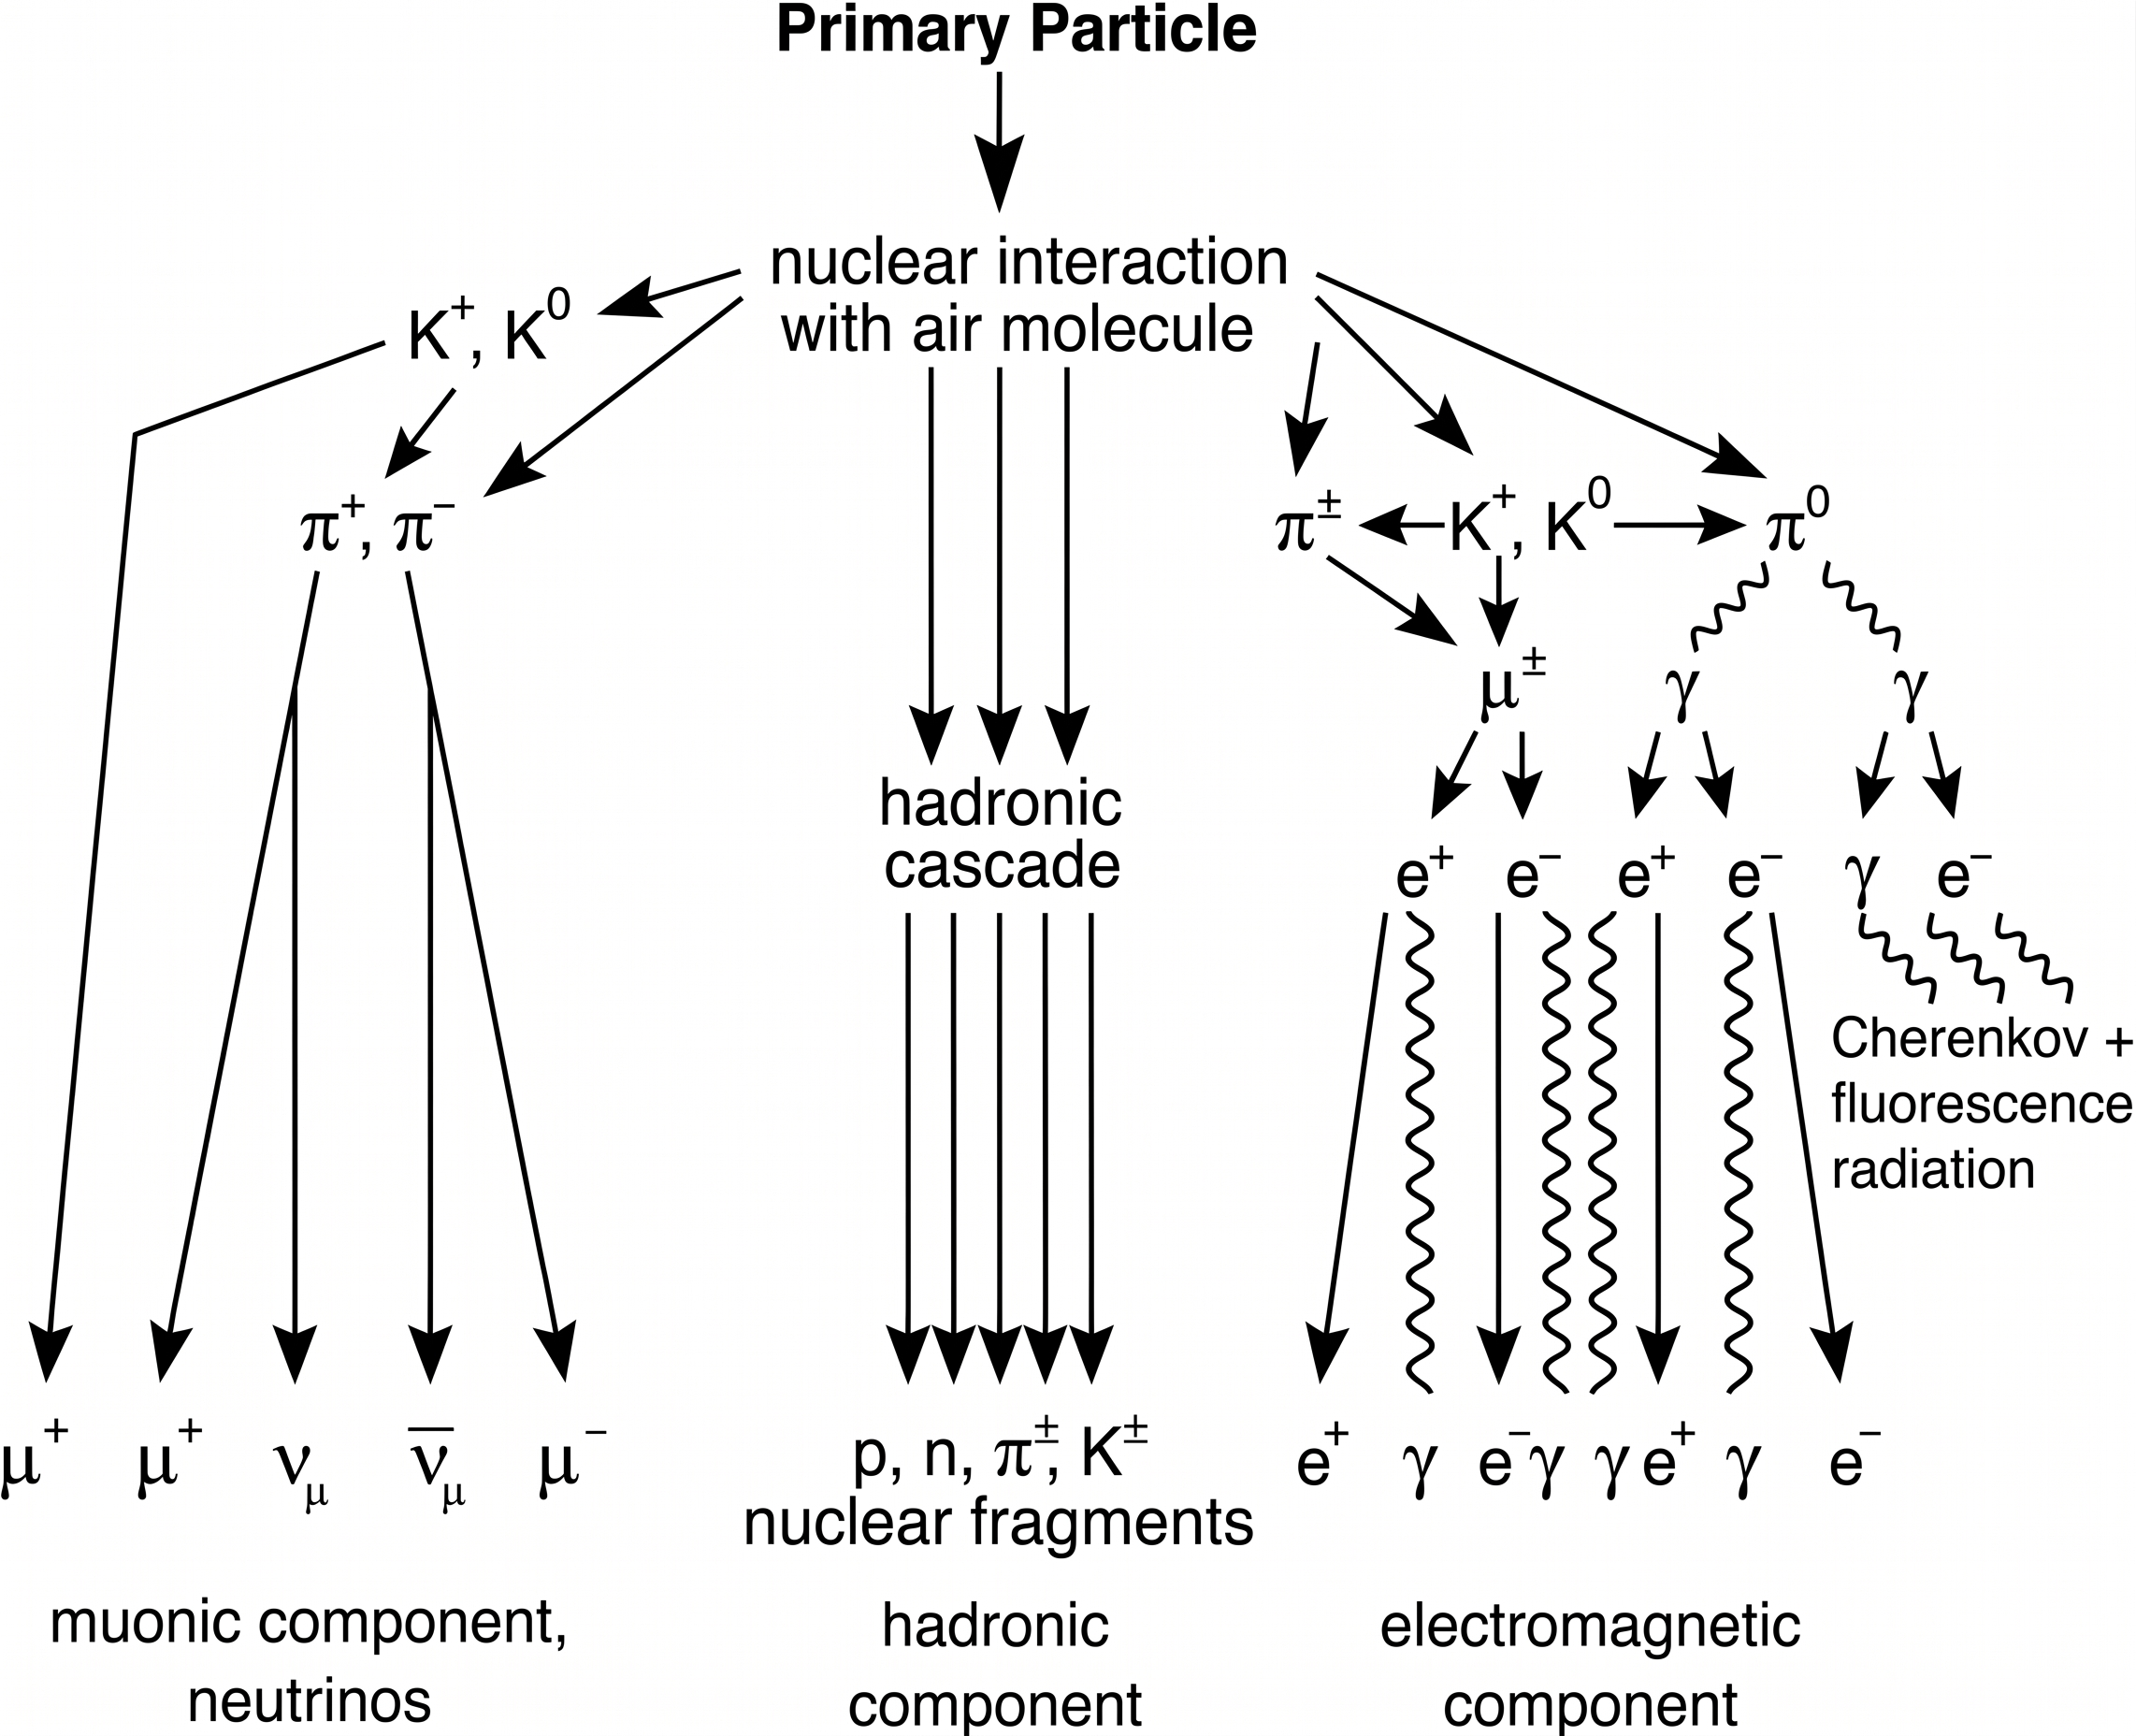
\includegraphics[width=0.85\linewidth]{figures/eas-diagram.png}
    \caption[Branching structure of an air shower.]{Branching structure of an air shower, grouped into the three components sampled at ground level. \textbf{Left:} the muonic and neutrino component. Charged kaons and pions ($K^{\pm}$, $K^{0}$, $\pi^{\pm}$) decay into muons and muon neutrinos, which are weakly interacting and reach the ground largely undisturbed. \textbf{Centre:} the hadronic component. Successive nuclear interactions sustain the hadronic cascade, whose surviving nucleons and mesons ($p$, $n$, $\pi^{\pm}$, $K^{\pm}$) constitute the nuclear fragments that reach the ground. \textbf{Right:} the electromagnetic component. Neutral pions decay promptly into photon pairs, which alternate pair production and bremsstrahlung to build an electron-positron-photon cascade; this component is what a Cherenkov or fluorescence detector observes directly, and what dominates the particle count of the shower.}
    \label{fig:cascade_tree}
\end{figure}

\subsection{Electromagnetic Showers}
\label{subsec:electromagnetic_showers}

The simplest type of EAS is initiated by a high-energy photon or electron. When a photon of sufficient energy passes close to an atmospheric nucleus, it converts into an electron-positron pair in the screened Coulomb field of that nucleus. This process, known as pair production, requires a photon energy of at least twice the electron rest mass ($2 m_e c^2 \approx 1.022$ MeV) and relies on the nearby nucleus to absorb the recoil momentum so that energy and momentum are simultaneously conserved. Each member of the resulting pair is then deflected in the same nuclear fields and radiates a bremsstrahlung photon, which can in turn produce a further pair, and so on. The cascade multiplies rapidly, roughly doubling the particle number at each step, until the energy per particle is no longer sufficient to sustain further pair production.

A useful framework for understanding this process is the Heitler model~\shortcite{heitler1984quantum, matthews2005heitler}, which describes the shower as a binary splitting process. After each splitting length, every particle splits into two secondaries of half the original energy. Starting from a primary of energy $E_0$, the shower reaches its maximum particle number when the energy per particle equals the critical energy $E_c$, below which ionization losses dominate over radiative processes. The number of generations required is $n = \log_2(E_0/E_c)$, so the maximum occurs at an atmospheric depth
\begin{equation}
    X_{\text{max}} = \frac{X_0}{\ln 2}\,\ln{\frac{E_0}{E_c}} \ ,
    \label{eq:xmax}
\end{equation}
measured in $\mathrm{g \ cm}^{-2}$ of traversed atmosphere, where $X_0$ is the radiation length\footnote{The radiation length is the mean atmospheric depth over which a high-energy electron loses all but a fraction $1/e$ of its energy through bremsstrahlung; it is the natural length scale of electromagnetic shower development.} and the factor $X_0/\ln 2$ is the effective splitting length of the cascade. The quantity $X_{\text{max}}$ is one of the most important observables in EAS physics: it depends logarithmically on the primary energy and is sensitive to the primary particle type, making it a key discriminant between electromagnetic and hadronic showers.

Shower development is tracked in units of \textit{atmospheric depth} rather than geometric distance, which is why $X_{\text{max}}$ carries units of $\mathrm{g \ cm}^{-2}$. Atmospheric depth is the mass of air per unit area contained in the column above a given point, and it is the natural coordinate for a cascade because the number of interactions a particle undergoes depends on how much matter it has crossed and not on how far it has moved. Appendix~\ref{sec:apx_depth} develops this in full, together with its two consequences for this work: the dependence of the traversed depth on the zenith angle, and the advantage of a high-altitude observation site.

\subsection{Hadronic Showers}
\label{subsec:hadronic_showers}

Showers initiated by protons or heavier nuclei are considerably more complex. The primary particle interacts inelastically with an atmospheric nucleus, producing a large multiplicity of secondary hadrons, predominantly pions. Charged pions $\pi^\pm$ continue the hadronic cascade through further inelastic interactions, while neutral pions $\pi^0$ decay almost immediately into photon pairs, seeding electromagnetic sub-showers at every generation. A hadronic shower is therefore a composite structure: a hadronic core that continuously feeds energy into a superposition of electromagnetic cascades developing at different depths.

This composite structure has two important consequences for detection. First, hadronic showers are intrinsically wider and more irregular in their lateral extent than purely electromagnetic showers, because hadronic interactions transfer significant transverse momentum and the multiple electromagnetic sub-showers develop independently along different axes. Second, a fraction of the primary energy is carried away by neutrinos produced in charged pion and muon decay, making hadronic showers less efficient at producing detectable particles at ground level than gamma-induced showers of the same primary energy. These morphological and energetic differences form the physical basis for gamma-hadron discrimination~\shortcite{rao1998extensive}.

Figure~\ref{fig:proton_vs_photon} illustrates these differences at the level of the ground detector array. The average footprint of gamma-induced showers is more compact and concentrated near the shower core, while proton-induced showers exhibit a broader, less symmetric lateral distribution and higher particle counts at peripheral detectors. The difference map (right panel) highlights the core-dominated excess for gamma events and the extended halo for hadronic events, providing a direct visual foundation for the morphological discrimination task.

\begin{figure*}[ht!]
    \centering
    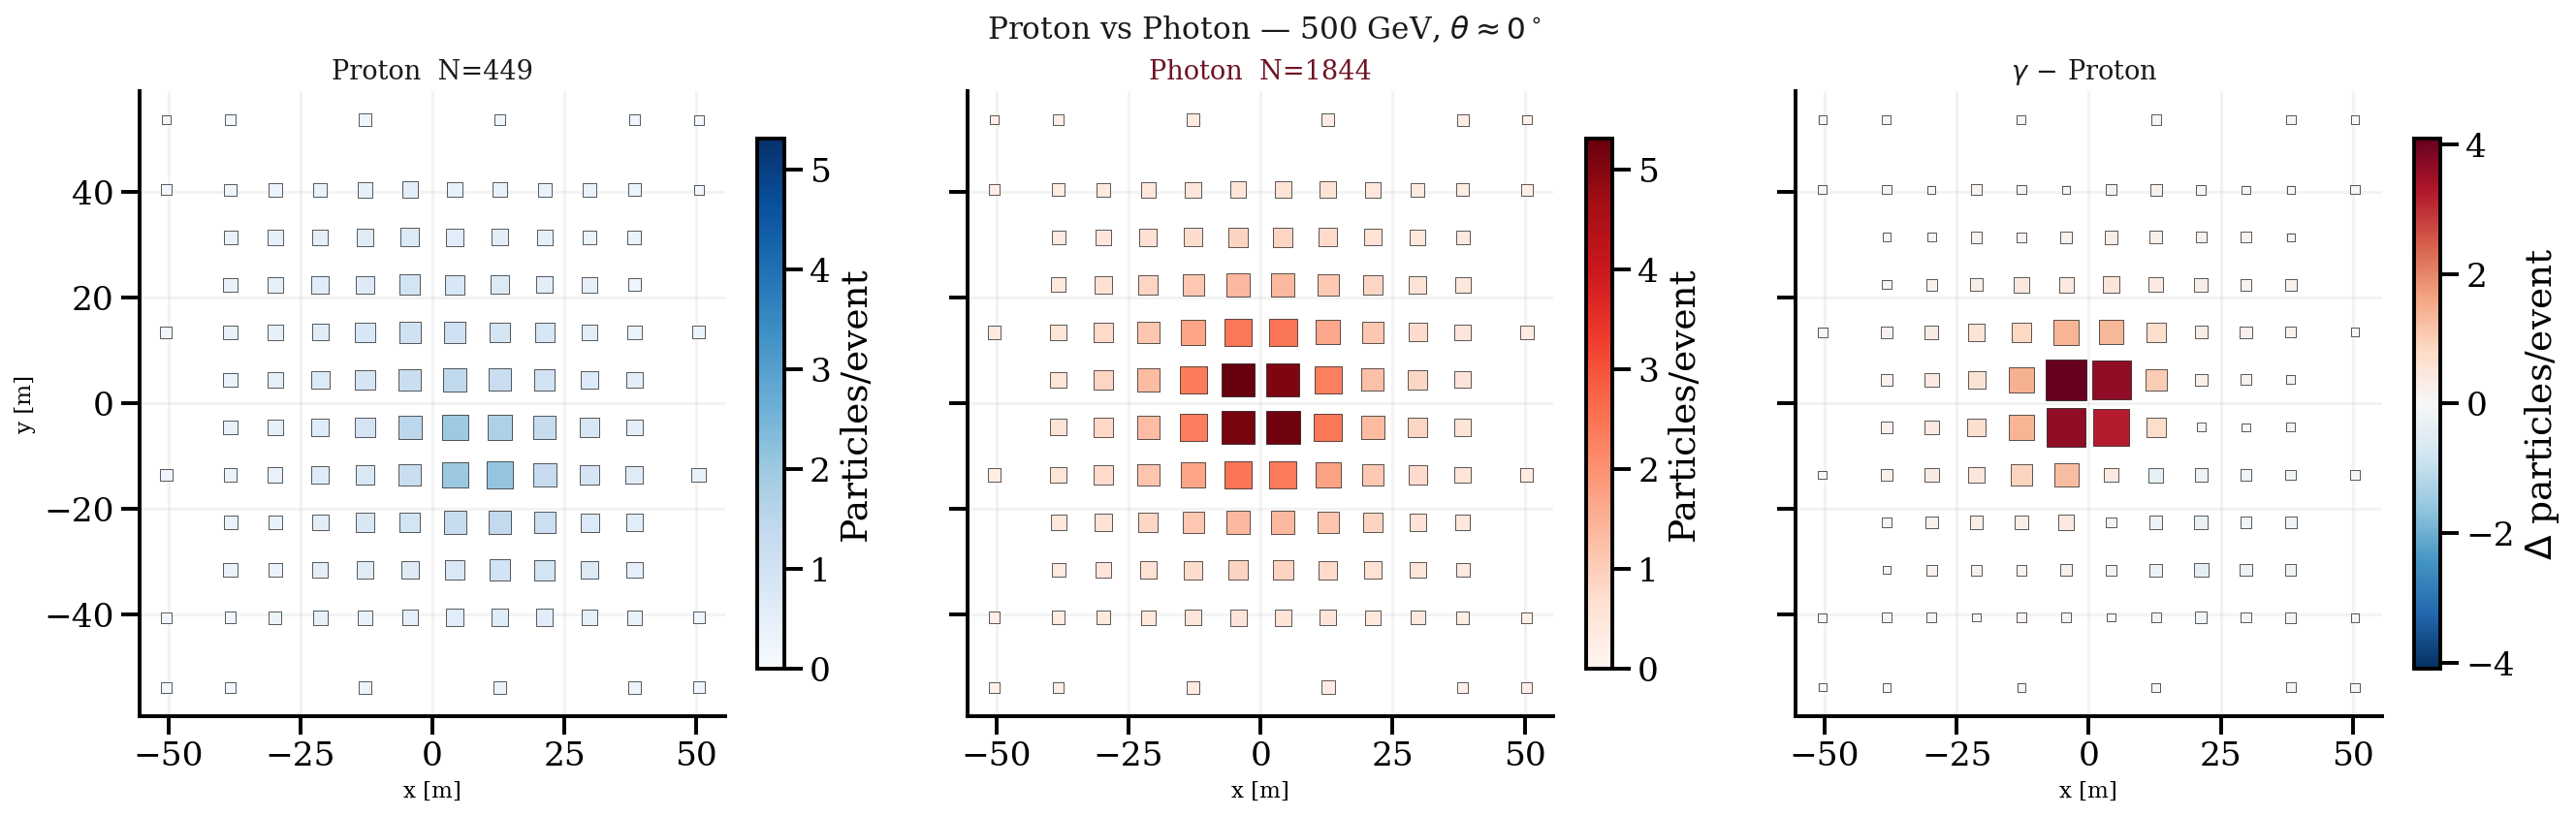
\includegraphics[width=1\linewidth]{figures/eas_proton_vs_photon.png}
    \caption[Average shower footprint: proton vs photon comparison.]{Average shower footprint at 500 GeV and $\theta \approx 0\degree$. \textbf{Left:} mean particle count per detector for proton-induced showers. \textbf{Center:} mean particle count per detector for gamma-induced showers. \textbf{Right:} difference map ($\gamma$ $-$ proton), revealing the more compact core signature of electromagnetic showers versus the wider lateral spread of hadronic showers. Marker size is proportional to particle count; position corresponds to physical detector location on the array.}
    \label{fig:proton_vs_photon}
\end{figure*}

\subsection{Shower Observables}

At ground level, an EAS manifests as a propagating disk of particles sweeping across the detector array and leaving a spatiotemporal pattern of hits. The key observables recorded by a surface array are the number of particles at each detector, the deposited energy, and the arrival time of the shower front.

The lateral distribution describes how the density of secondary particles varies with the distance from the shower core at the detector altitude. For the electromagnetic component of a shower, this distribution is well approximated by the Nishimura-Kamata-Greisen (NKG) function~\shortcite{nishimura1958kamata},
\begin{equation}
    \rho (r) = \frac{N_e}{2\pi r^2_{M}}\frac{\Gamma(4.5 - s)}{\Gamma(s) \Gamma(4.5-2s)}\qty(\frac{r}{r_M})^{s-2}\qty(1+\frac{r}{r_M})^{s-4.5},
    \label{eq:nkg}
\end{equation}
where $N_e$ is the total number of electrons, $r$ is the distance from the shower core, $r_M$ is the Molière radius,\footnote{The Molière radius is the characteristic transverse scale of an electromagnetic shower, defined as the radius of the cylinder around the shower axis that contains, on average, about 90\% of the deposited energy; it sets the lateral width of the particle distribution.} and $s$ is the shower age parameter that tracks the developmental stage of the cascade ($s = 1$ at shower maximum). The NKG function is relevant here as the classical parametric description of the lateral distribution: traditional reconstruction pipelines fit it to the measured hit pattern to estimate the shower size and core position. The deep learning model developed in this thesis does not fit any fixed functional form; instead, it learns the lateral and temporal structure of the shower directly from the detector hits, and therefore does not assume the shape given by the NKG function in advance. Figure~\ref{fig:lateral_distribution} shows the distribution predicted by this function.

\begin{figure*}[ht!]
    \centering
    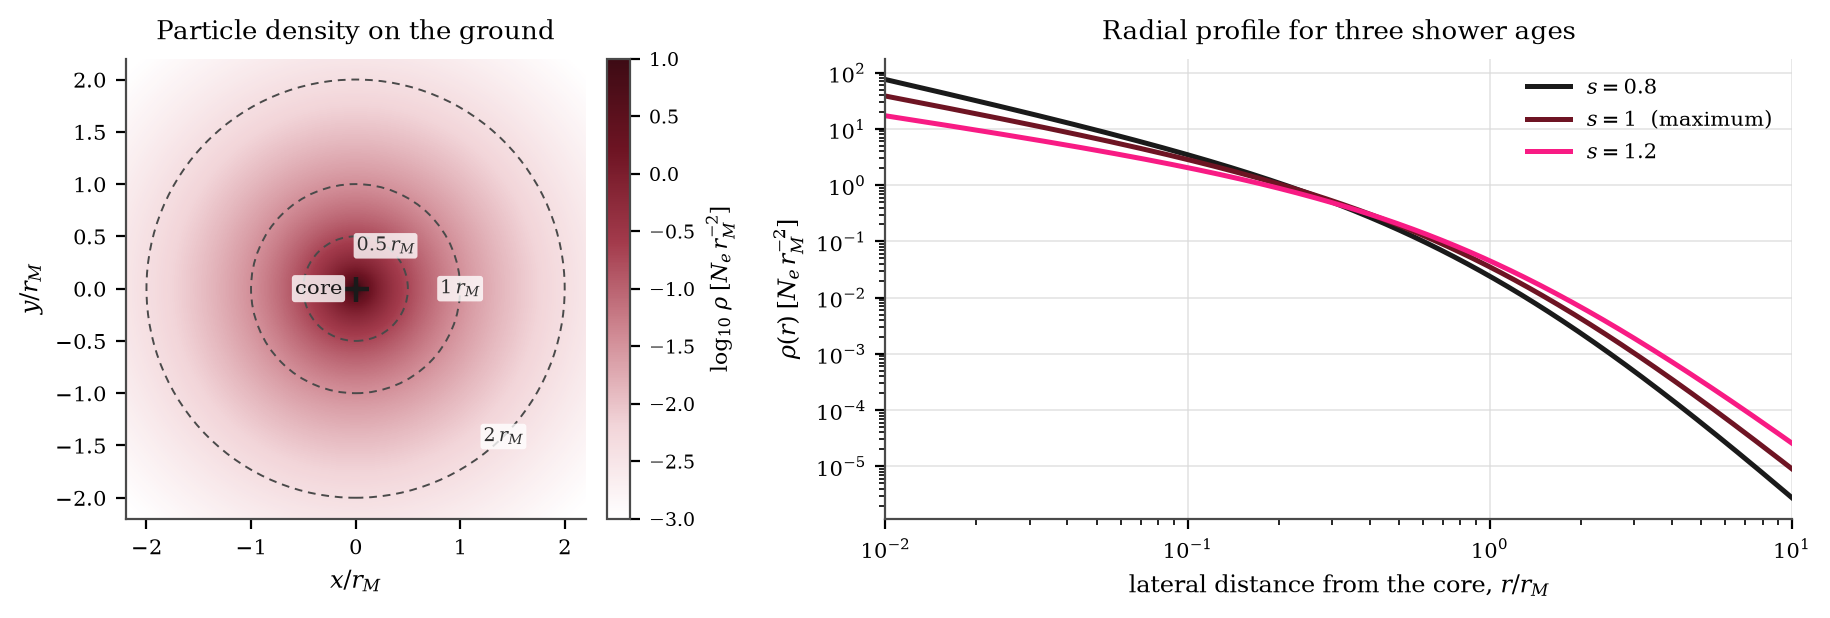
\includegraphics[width=1\linewidth]{figures/lateral_distribution.png}
    \caption[Lateral particle density predicted by the NKG function.]{Lateral particle density predicted by the NKG function of Equation~\ref{eq:nkg}, in units of the Moli\`ere radius $r_M$ so that it does not depend on the air density at the observation altitude. \textbf{Left:} density on the ground at shower maximum ($s = 1$), with rings at $0.5$, $1$ and $2\,r_M$. \textbf{Right:} radial profile for three shower ages: a young shower is more concentrated on the core, an older one flatter and wider.}
    \label{fig:lateral_distribution}
\end{figure*}

The timing of the shower front encodes the arrival geometry of the primary particle. As shown in Figure~\ref{fig:shower_geometry}, for an ideal planar front traveling at the speed of light, the arrival time difference between two detectors separated by a displacement vector $\Delta \textbf{r}$ is
\begin{equation}
    \Delta t = -\frac{\hat{n}\cdot \Delta \textbf{r}}{c},
    \label{eq:front}
\end{equation}
where $\hat{n}$ is the unit vector in the shower propagation direction. In practice, shower front curvature and stochastic fluctuations introduce deviations from this ideal model, but the timing information remains the primary observable for reconstructing the arrival direction of the incoming primary. In this thesis the azimuthal angle is held fixed in the simulations (Section~\ref{sec:corsika}), so the arrival-time gradient is exploited specifically for the reconstruction of the zenith angle $\theta$ --- one of the three target tasks of the model --- which is why this observable is emphasized here.

\begin{figure*}[ht!]
\centering
\begin{tikzpicture}[scale=0.92]

% ---- panel (a): three-dimensional view of the arrival direction ----
\begin{scope}[
    x={(1cm,-0.26cm)}, y={(0.60cm,0.36cm)}, z={(0cm,1cm)},
    scale=0.62]

  \fill[gray!10] (0,0,0) -- (6,0,0) -- (6,5,0) -- (0,5,0) -- cycle;
  \draw[gray!45, very thin]
    \foreach \i in {0,1,2,3,4,5,6} { (\i,0,0) -- (\i,5,0) }
    \foreach \j in {0,1,2,3,4,5} { (0,\j,0) -- (6,\j,0) };
  \draw[gray!60] (0,0,0) -- (6,0,0) -- (6,5,0) -- (0,5,0) -- cycle;

  \draw[dashed, gray!70, -{Stealth[length=2mm]}] (3,2.5,0) -- (3,2.5,5.0)
      node[above, font=\footnotesize, black] {zenith};

  \draw[very thick, -{Stealth[length=2.6mm]}]
      (5.20,4.34,4.09) -- (3,2.5,0);
  \node[font=\footnotesize, anchor=west] at (5.35,4.5,4.3) {shower axis};

  \draw[dashed, gray!70] (5.20,4.34,0) -- (3,2.5,0);
  \draw[dashed, gray!40] (5.20,4.34,4.09) -- (5.20,4.34,0);

  \draw[gray!70, -{Stealth[length=2mm]}] (3,2.5,0) -- (5.8,2.5,0)
      node[right, font=\footnotesize, black] {$x$};

  \draw[thick] plot coordinates {(3.000,2.500,1.350) (3.049,2.541,1.349) (3.097,2.581,1.344) (3.146,2.622,1.337) (3.194,2.662,1.326) (3.241,2.702,1.313) (3.288,2.741,1.297) (3.335,2.780,1.277) (3.381,2.818,1.256) (3.425,2.856,1.231) (3.469,2.893,1.203) (3.512,2.928,1.173) (3.554,2.963,1.141) (3.595,2.997,1.105)};
  \node[font=\small] at (3.427,2.857,1.764) {$\theta$};

  \draw[thick] plot coordinates {(4.450,2.500,0.000) (4.448,2.578,0.000) (4.442,2.655,0.000) (4.431,2.732,0.000) (4.417,2.808,0.000) (4.398,2.884,0.000) (4.376,2.958,0.000) (4.349,3.031,0.000) (4.319,3.103,0.000) (4.285,3.172,0.000) (4.247,3.240,0.000) (4.205,3.306,0.000) (4.160,3.369,0.000) (4.112,3.430,0.000)};
  \node[font=\small] at (4.645,3.097,0) {$\varphi$};

  \fill (3,2.5,0) circle (2.0pt);
  \node[font=\footnotesize, anchor=east] at (2.85,2.5,0) {core};
\end{scope}
\node[font=\small] at (2.55,-2.05) {(a) arrival direction};

% ---- panel (b): side view of the shower front ----
\begin{scope}[xshift=6.9cm, yshift=-0.55cm, scale=0.80]

  \draw[gray!60] (0.1,0) -- (7.0,0);
  \fill[black] (0.95,0) rectangle ++(0.5,0.22);
  \node[font=\footnotesize, below] at (1.20,-0.04) {A};
  \fill[black] (4.15,0) rectangle ++(0.5,0.22);
  \node[font=\footnotesize, below] at (4.40,-0.04) {B};

  \draw[dashed, gray!70] (5.9,0) -- (5.9,3.9)
      node[above, font=\footnotesize, black] {zenith};

  \draw[very thick, -{Stealth[length=2.6mm]}] (3.9,3.46) -- (5.9,0);
  \node[font=\footnotesize, anchor=south east] at (4.05,3.42) {shower axis};

  \draw[thick] (5.9,2.1) to[bend right=16] (4.99,1.52);
  \node[font=\small] at (5.35,2.05) {$\theta$};

  \draw[very thick] (1.20,0) -- (5.10,2.25);
  \node[font=\footnotesize, anchor=west] at (1.15,2.30) {shower front};
  \draw[gray!70, thin] (1.95,2.15) -- (2.35,0.66);

  \draw[{Stealth[length=2mm]}-{Stealth[length=2mm]}, thick] (4.40,0.24) -- (3.704,1.446);
  \node[font=\small, anchor=west] at (4.16,0.88) {$c\,\Delta t$};

  \draw[|<->|, gray!70] (1.20,-0.95) -- (4.40,-0.95);
  \node[font=\small, below] at (2.80,-0.93) {$\Delta \mathbf{r}$};
\end{scope}
\node[font=\small] at (9.7,-2.05) {(b) arrival-time gradient};

\end{tikzpicture}
\caption[Arrival geometry of an extensive air shower.]{Arrival geometry of an extensive air shower. \textbf{(a)} The direction of the primary is given by the zenith angle $\theta$, from the vertical, and the azimuth $\varphi$, on the plane of the array; the axis meets that plane at the core. \textbf{(b)} Side view. The front is perpendicular to the axis, so it reaches A first and still has $c\,\Delta t$ to travel before reaching B; that delay is the projection of their separation onto the direction of propagation, Equation~\ref{eq:front}. Here $\varphi$ is fixed at $0\degree$ (Section~\ref{sec:corsika}), so only $\theta$ is reconstructed.}
\label{fig:shower_geometry}
\end{figure*}

Figure~\ref{fig:angle_evolution} shows how the average shower footprint evolves with the zenith angle for 500 GeV proton-induced showers simulated at CONDOR. As $\theta$ increases, the footprint elongates along the projection of the shower axis onto the detector plane, the lateral spread widens, and the arrival-time gradient across the array steepens. These systematic morphological changes underlie the angular reconstruction task addressed in this thesis.

\begin{figure*}[ht!]
    \centering
    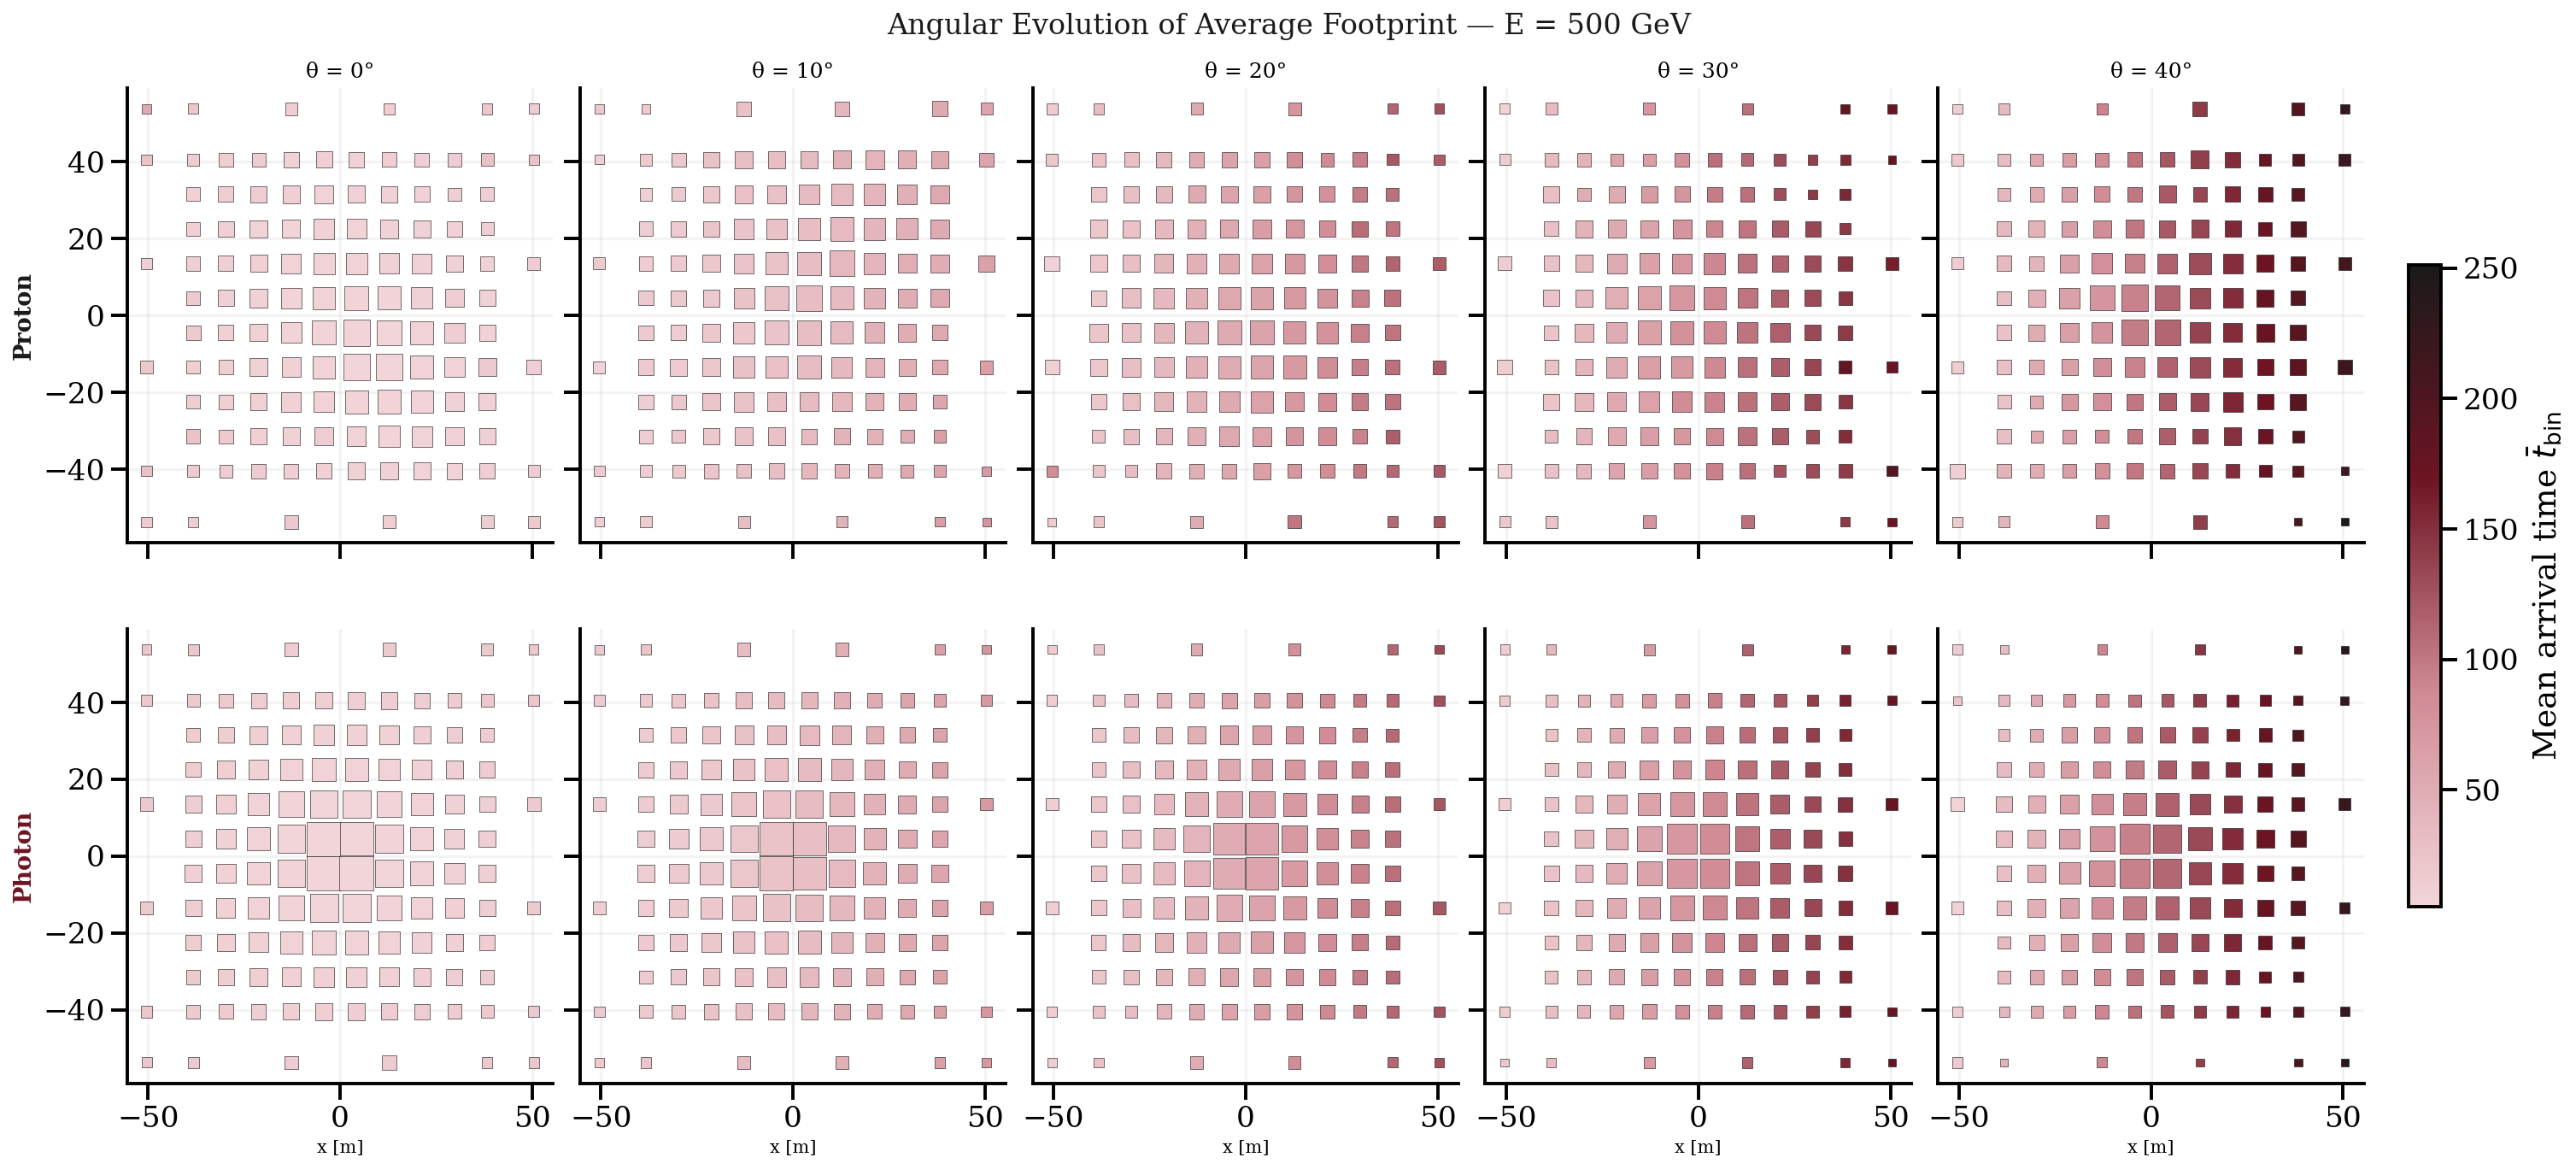
\includegraphics[width=1\linewidth]{figures/eas_angle_evolution.png}
    \caption[Angular evolution of the average EAS footprint.]{Angular evolution of the average shower footprint for proton-induced events at $E = 500\,\text{GeV}$. Each panel shows the mean particle count per detector averaged over all events within the corresponding zenith angle bin ($\theta \approx 0\degree$, $10\degree$, $20\degree$, $30\degree$, $40\degree$). As the zenith angle increases, the shower footprint elongates along the projected shower axis and the lateral spread broadens, providing the morphological signature exploited for zenith angle reconstruction. Color encodes the mean arrival time $\bar{t}_\mathrm{bin}$; marker size is proportional to particle count.}
    \label{fig:angle_evolution}
\end{figure*}

\section{Ground-Based Detection of EAS}

Ground-based observatories exploit the EAS as an indirect measurement device: rather than detecting the primary particle directly, they sample the shower footprint at ground level and use the recorded hit pattern to infer the properties of the primary cosmic ray, such as its type, energy, and arrival direction. This approach enables observation over large sky areas simultaneously and is not limited by collection area in the way that satellite detectors are.

In the sub-TeV and TeV energy regimes, ground-based arrays fall into two dominant technology categories. Water Cherenkov detectors, used by observatories such as HAWC~\shortcite{HAWK} and LHAASO~\shortcite{cao2022largehighaltitudeair}, consist of large tanks of purified water in which secondary particles produce Cherenkov light\footnote{Cherenkov light is the faint electromagnetic radiation emitted when a charged particle traverses a medium faster than the local phase velocity of light in that medium; its intensity and angular profile encode the particle's velocity and direction.} recorded by photomultiplier tubes. They offer good muon sensitivity, which is advantageous for gamma-hadron discrimination, but require large structural investment at high altitude. The same technology has been adopted for the Southern Wide-field Gamma-ray Observatory (SWGO)~\shortcite{SWGO}, a next-generation array proposed for the southern hemisphere, which would extend this coverage to a sky region that HAWC and LHAASO cannot observe. Plastic scintillator arrays, used by operating observatories such as Tibet AS$\gamma$~\shortcite{amenomori2019first} and adopted for the future CONDOR array~\shortcite{arratia2025condor}, consist of segmented scintillator panels that produce light pulses when charged particles pass through them, read out by silicon photomultipliers (SiPMs) through wavelength-shifting fibers. Scintillator arrays offer better timing resolution, higher modularity, and lower deployment weight than water Cherenkov detectors, making them suitable for operation at the highest altitudes.

\section{The CONDOR Observatory}
\label{sec:condor_observatory}

The CONDOR (\textbf{CO}mpact \textbf{N}etwork of \textbf{D}etectors with \textbf{O}rbital \textbf{R}ange) observatory is a proposed high-altitude gamma-ray and cosmic ray array designed to observe EAS in the 100 GeV to 1 TeV range~\shortcite{arratia2025condor}. It is currently in its design and validation phase, so all data used in this thesis are generated through Monte Carlo simulations that reproduce the expected response of the CONDOR array under its planned high-altitude operating conditions; the simulation framework is described in detail in Section~\ref{sec:corsika}. Figure~\ref{fig:condor-array} shows a schematic representation of the array layout.

\begin{figure}[ht!]
    \centering
    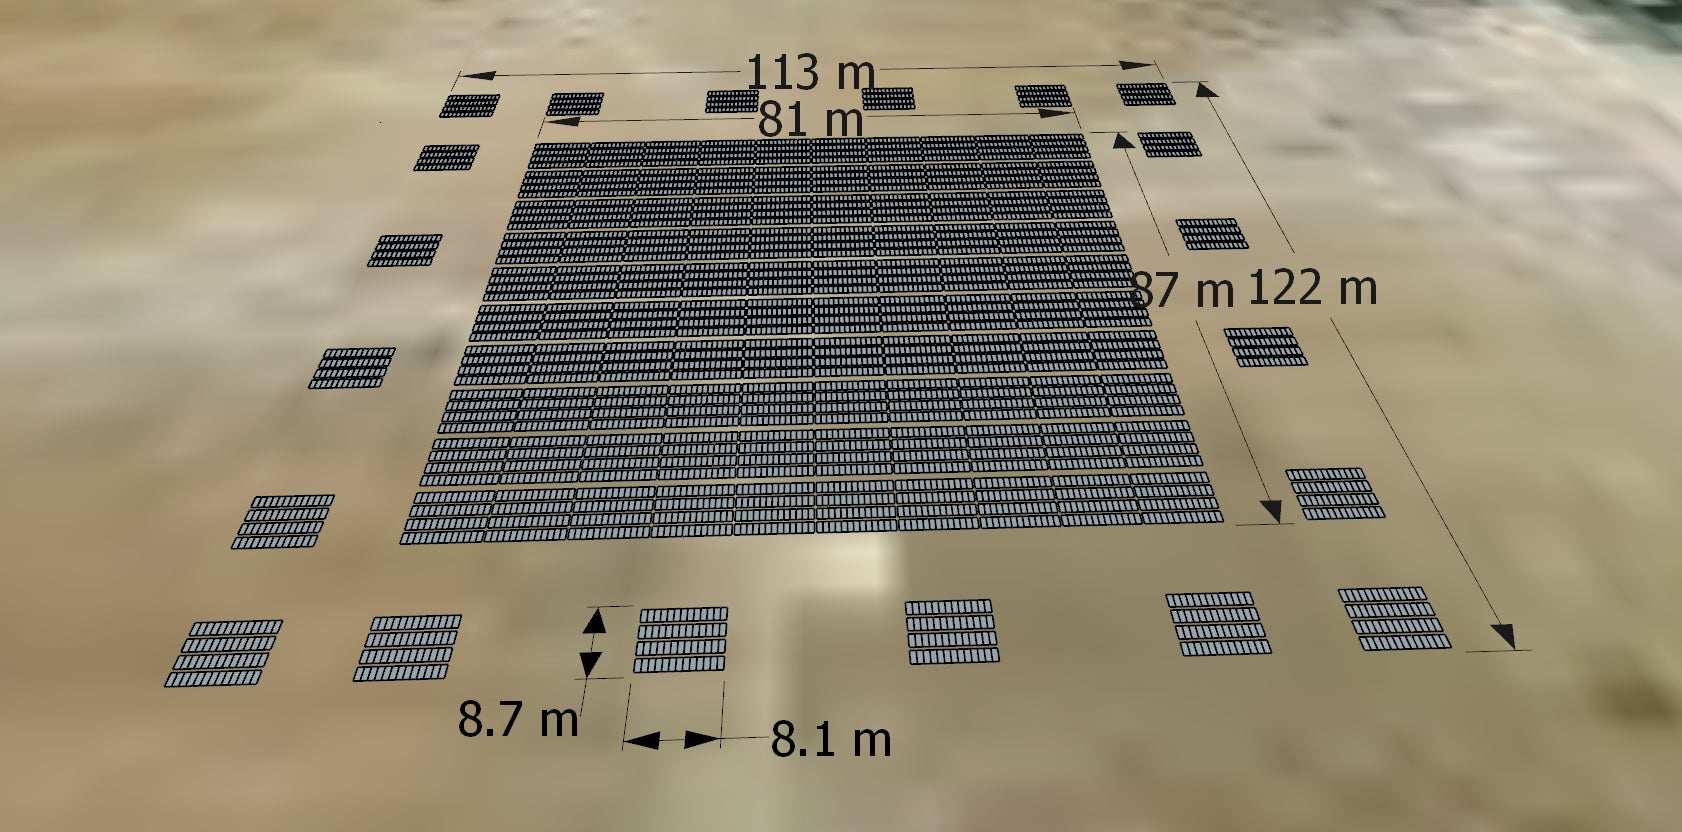
\includegraphics[width=0.95\linewidth]{figures/condor_img_2.png}
    \caption[Schematic of the CONDOR detector array layout.]{Schematic representation of the CONDOR observatory layout. The array achieves a high fill factor in its inner region using thousands of plastic scintillator units, surrounded by an outer veto ring to suppress backgrounds. Source: CONDOR Observatory~\shortcite{arratia2025condor}.}
    \label{fig:condor-array}
\end{figure}

\subsection{Design and High-Altitude Advantage}

CONDOR will be located within the Atacama Astronomical Park at Cerro Toco, Chile, at an altitude of 5,300 meters above sea level, placing it above established facilities such as HAWC at 4,100 m and LHAASO at 4,410 m. This altitude is the central design advantage of CONDOR. The number of secondary electrons reaching the ground level depends strongly on atmospheric depth: by operating closer to the shower maximum $X_{\text{max}}$, CONDOR avoids the progressive attenuation experienced by cascades traveling to lower elevations. This enables CONDOR to lower its effective energy threshold to approximately 100 GeV, accessing a range that is difficult to reach for lower-altitude arrays and that partially overlaps with the upper sensitivity limit of space-based gamma-ray instruments such as the Fermi-LAT.

\subsection{Array Layout and Detector Architecture}

The CONDOR array consists of 5,300 plastic scintillator detector units arranged in a compact central grid covering an area of approximately 6,000 $\mathrm{m}^2$, supplemented by 1,040 additional peripheral units forming a veto ring that encloses a total instrumented area of 14,000 $\mathrm{m}^2$. The central region achieves a fill factor of 90\%, meaning that nearly the entire surface is actively sensitive to shower particles. This high fill factor is essential for low-energy operation, where the shower footprint is small and sparse hits must be captured efficiently.

For the purpose of simulation and reconstruction, these individual detector units are grouped into \textbf{detector modules}, each covering an area of approximately $8.1 \times 8.7~\mathrm{m}^2$. As shown in Figure~\ref{fig:condor-modules}, the full array comprises 120 modules: 100 arranged in a $10 \times 10$ central grid, plus 20 peripheral modules. Each module aggregates the signals from its constituent scintillator panels into a single readout channel.

\begin{figure}[ht!]
    \centering
    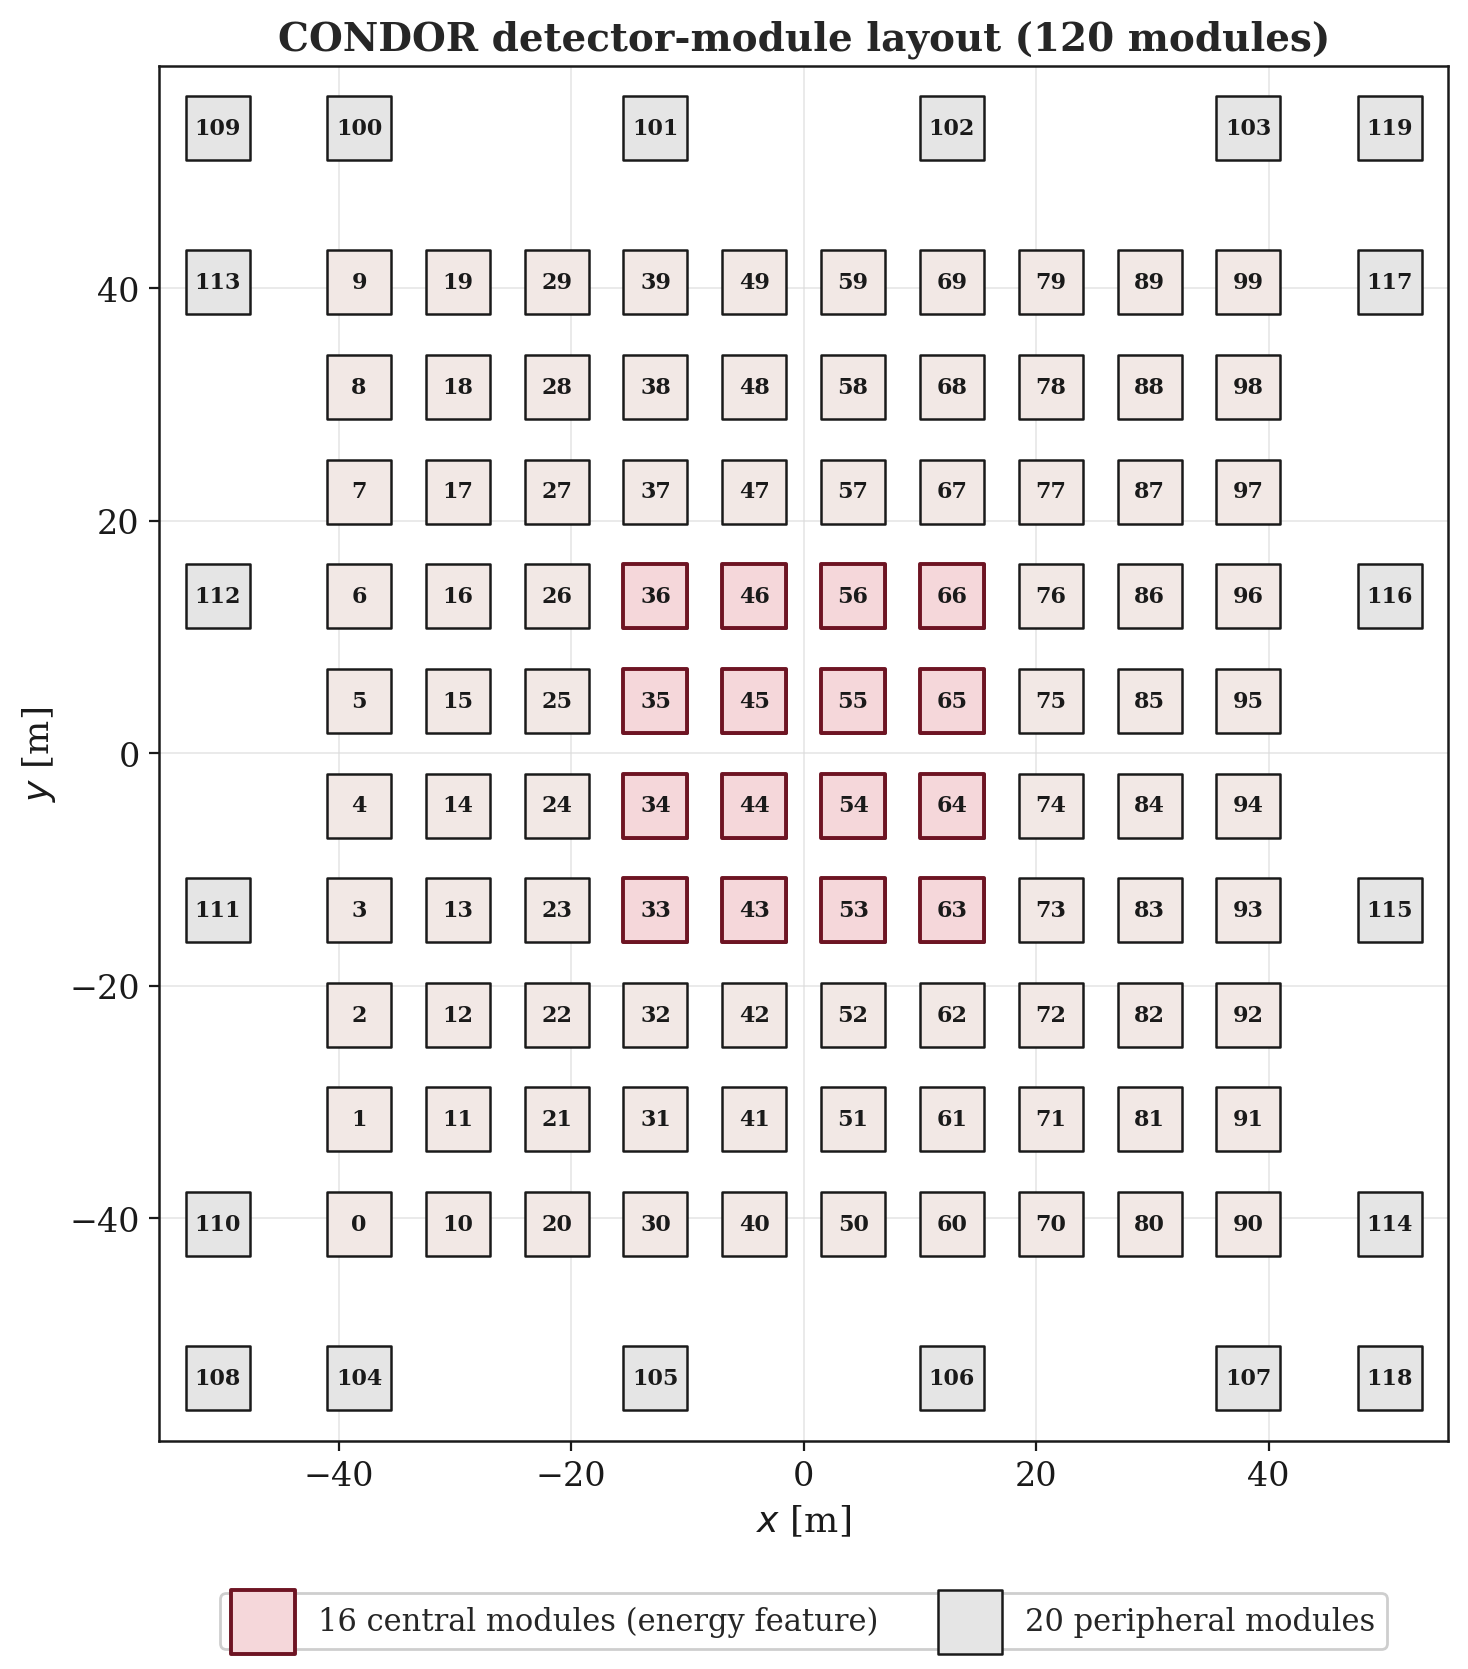
\includegraphics[width=0.85\linewidth]{figures/condor_modules_grid.png}
    \caption[Simulated CONDOR detector-module geometry and identifiers.]{Simulated CONDOR detector-module geometry used throughout this thesis. The 100 central modules (identifiers 0--99) form a $10 \times 10$ grid spanning approximately $87 \times 81~\mathrm{m}^2$, surrounded by 20 peripheral modules (identifiers 100--119), matching the planned observatory configuration. Each module aggregates the signals of its constituent scintillator units into a single readout channel. The module identifier is used directly as the \texttt{detector\_id} input feature of the model.}
    \label{fig:condor-modules}
\end{figure}

It is important to distinguish the two levels at which the shower is represented. The CORSIKA simulation itself does not know about detector modules: it tracks the air shower as individual particles and records their type, energy, and arrival position and time at the ground. The mapping onto the 120 detector modules is performed afterwards, during the data-processing stage, where the raw particle hits falling within each module's footprint are aggregated into the per-module quantities used by the model (Chapter~\ref{ch:methodology}). Throughout this thesis, the term \textit{detector} therefore refers to these modules unless otherwise specified, and the analysis operates at the module level rather than at the level of individual scintillator units or raw particle hits.

Each detector unit consists of extruded plastic scintillator bars, each coated with a 0.25 $\mathrm{mm}$ layer of titanium dioxide to enhance internal light reflection. A wavelength-shifting optical fiber runs through a central hole in each bar, collecting the fluorescent light produced by ionizing particles and guiding it to a silicon photomultiplier. The chosen SiPM model, the Hamamatsu S14160-6015PS, features 159,565 pixels and a photon detection efficiency of 32\%, providing single-photon sensitivity and precise timing. The units are enclosed in 5 $\mathrm{mm}$ aluminum housings for protection against the harsh Atacama environment, including the large daily temperature variations that require remote bias voltage adjustments to maintain stable detector performance.

\subsection{Data Acquisition and Sub-Nanosecond Synchronization}

Reconstructing the arrival direction of a shower front traveling at nearly the speed of light requires timing accuracy across thousands of detector nodes separated by tens to hundreds of meters. The intrinsic time resolution of each CONDOR unit is designed to be below one nanosecond, and sub-nanosecond synchronization across the full array is therefore a system-level requirement.

CONDOR is designed to achieve this through White Rabbit technology~\shortcite{moreira2009white}, an Ethernet-based timing protocol based on the IEEE 1588 standard\footnote{IEEE 1588, also known as the Precision Time Protocol (PTP), is an international standard for synchronizing clocks across nodes of a packet-switched network to sub-microsecond accuracy.} that distributes a pulse-per-second signal derived from the Global Positioning System (GPS) through fiber optic cables to White Rabbit nodes distributed across the array. Each node serves approximately ten detector panels, providing sub-nanosecond timing to each readout board. This synchronization allows offline discrimination between genuine shower hits and uncorrelated dark noise pulses, and it is the foundation on which the timing-based reconstruction of arrival direction depends.

\section{The CORSIKA Simulation Framework}
\label{sec:corsika}

Because the CONDOR observatory has not yet begun scientific operations, all data used in this thesis are generated through Monte Carlo simulation. The simulation tool is CORSIKA (COsmic Ray SImulations for KAscade), developed at the Karlsruhe Institute of Technology and the standard framework for EAS simulation across the ground-based cosmic ray and gamma-ray community~\shortcite{Heck1998}.

CORSIKA tracks the propagation, interaction, and decay of every secondary particle produced in the cascade, from the first interaction of the primary in the upper atmosphere down to a configurable observation level. The cascade is treated as a set of coupled components --- hadronic, electromagnetic, and muonic --- each governed by the relevant physics. Hadronic interactions are split into two energy regimes handled by different interaction models matched at a transition energy. The high-energy regime --- the first, most energetic collisions of the primary and its leading secondaries --- is simulated with the EPOS model~\shortcite{pierog2009epos}, which provides a comprehensive treatment of minijet production, string fragmentation, and nuclear effects. The low-energy regime --- the more numerous, softer interactions that dominate the later stages of shower development --- is handled by the GHEISHA model~\shortcite{fesefeldt1985gheisha}. The neutral pions produced in these hadronic interactions decay almost immediately into photon pairs and feed the electromagnetic component, whose pair-production and bremsstrahlung sub-cascades are followed explicitly down to user-defined energy thresholds, below which particles are no longer tracked. The atmosphere is modeled as a series of layers with exponentially varying density, and the observation level is set to 5,300 m above sea level to match the planned altitude of CONDOR.

Conceptually, CORSIKA provides a full Monte Carlo realization --- with all the stochastic fluctuations of real showers --- of the average cascade development captured analytically by the Heitler model introduced earlier in this chapter. Whereas the Heitler model yields the mean depth of shower maximum and the mean particle number as smooth functions of primary energy, CORSIKA samples individual showers event by event, reproducing the shower-to-shower variability and the correlations between observables that the reconstruction model must learn to exploit.

The simulations cover proton and gamma-ray primaries at three discrete energies, 300, 500, and 800 GeV, with zenith angles sampled at uniform intervals from $0\degree$ to $40\degree$ in steps of $2\degree$, producing 21 discrete inclinations, and the azimuthal angle fixed at $\phi = 0\degree$. Events producing fewer than 30 secondary particles at the observation level are discarded. The full dataset construction and balancing procedure is described in Chapter~\ref{ch:methodology}.

\section{Convolutional Neural Networks}

Convolutional neural networks (CNNs) are a class of deep learning architectures designed to process data with local spatial or temporal structure~\shortcite{lecun1998convolutional}. Their defining property is the use of shared learned filters applied across the input, which allows the network to detect the same local pattern regardless of where it appears in the sequence. In this thesis, a CNN backbone is used to extract local temporal features from the ordered sequence of detector hits that constitutes the primary input to the reconstruction model.

\textbf{The convolution operation.} For a one-dimensional input sequence $\textbf{x} \in \mathbb{R}^{T\times C_{\text{in}}}$, where $T$ is the sequence length and $C_{\text{in}}$ is the number of input channels, and a learned filter $\textbf{w} \in \mathbb{R}^{k\times C_{\text{in}}\times C_{\text{out}}}$ of kernel size $k$, the output at position $t$ for output channel $j$ is
\begin{equation}
    y_j(t) = \sum_{c=1}^{C_\text{in}} \sum_{i=0}^{k-1} w_{i,c,j} \cdot x_{t+i,c} + b_j,
\end{equation}
where $b_j$ is learnable bias. The filter $\textbf{w}$ is shared across all positions $t$, which gives CNNs two important properties: translational equivariance, meaning that a pattern detected at one position will also be detected if it appears elsewhere in the sequence, and a substantially reduced parameter count compared to a fully connected network operating on the same input.

\textbf{Pooling and normalization.} Following each convolution, max pooling reduces the temporal resolution by selecting the maximum activation within non-overlapping windows of size $p$,
\begin{equation}
    z_j(t) = \max_{0\leq i <p}{ y_j (tp +i)} \ ,
\end{equation}
retaining the presence and magnitude of detected features while discarding fine positional detail. Batch normalization~\shortcite{ioffe2015batch} then standardizes each feature map across the batch dimension before applying learnable scale and shift parameters,
\begin{equation}
    \hat{y}_j = \frac{y_j - \mu_j}{\sqrt{\sigma^2_j + \epsilon}}, \quad \tilde{y}_j = \gamma_j \hat{y}_j + \beta_j
\end{equation}
where $\mu_j$ and $\sigma^2_j$ are the batch mean and variance for channel $j$, and $\gamma_j, \beta_j$ are trainable. Batch normalization stabilizes training and permits higher learning rates without destabilizing the optimization. It was originally motivated as a way to reduce internal covariate shift, although subsequent work attributes its effect primarily to a smoothing of the optimization landscape rather than to covariate-shift reduction.

\textbf{Activation.} The nonlinearity applied after normalization is the Exponential Linear Unit (ELU)~\shortcite{clevert2015fast},

\begin{equation}
    \text{ELU}(x) = \begin{cases}
        x & \text{if} \ x >0 , \\
        \alpha(e^x - 1) & \text{if} \ x \leq 0,
    \end{cases}
\end{equation}
where the scale parameter $\alpha$ controls the saturation value for negative inputs; the standard choice $\alpha = 1$ is used, which makes the activation continuously differentiable at $x = 0$ (the left derivative $\alpha e^{x}|_{x=0} = \alpha$ matches the right derivative of $1$) and sets the negative saturation level to $-1$. Unlike the rectified linear unit (ReLU), ELU produces negative outputs for negative inputs, preserving a non-zero mean activation and accelerating convergence in deep networks by reducing the bias shift effect.

The specific CNN architecture used in this work, including the number of layers, filter configurations, and projection heads, is detailed in Chapter~\ref{ch:methodology}.

\section{Transformer Architectures}
\label{sec:transformer}

The Transformer is a deep learning architecture introduced by~\shortciteA{vaswani2017attention} that processes sequences through scaled dot-product attention. Unlike recurrent architectures such as long short-term memory networks~\shortcite{hochreiter1997long}, which propagate information sequentially through a hidden state and struggle with long-range dependencies, the Transformer computes all pairwise interactions between sequence positions in parallel, making it both more expressive for long-range structure and more efficient on modern hardware. In this thesis, Transformer streams process both the CNN-extracted feature sequence and the raw masked hit sequence to capture global temporal dependencies across the full shower hit pattern; the full multi-stream configuration is detailed in Chapter~\ref{ch:methodology}.

\textbf{Scaled dot-product attention.} The input to the attention mechanism is a sequence of \textit{token embeddings}: vector representations of the discrete elements of the sequence (in this work, each token corresponds to one detector hit, encoded either as its raw feature vector or as a CNN-derived feature embedding). Three learned linear projections map this sequence to queries, keys, and values: the \textit{query} of a position asks ``what information am I looking for?'', the \textit{key} of every other position answers ``what information do I expose?'', and the \textit{value} carries the actual content that will be propagated. Concretely, the three projections produce $\textbf{Q} \in \mathbb{R}^{T \times d_k}$, $\textbf{K} \in \mathbb{R}^{T \times d_k}$, and $\textbf{V} \in \mathbb{R}^{T \times d_v}$, and the attention output is
\begin{equation}
    \text{Attention}(\textbf{Q}, \textbf{K}, \textbf{V}) = \text{softmax}\qty(\frac{\textbf{QK}^\top}{\sqrt{d_k}})\textbf{V}.
\end{equation}
The matrix $\textbf{QK}^{\top}/\sqrt{d_k}$ contains the scaled similarity score between every pair of positions. After the softmax, each row becomes a probability distribution over the sequence, and the output at each position is a weighted sum of the value vectors. The scaling by $1/\sqrt{d_k}$ prevents the dot products from growing large in magnitude as $d_k$ increases, which would push the softmax into regions of near-zero gradient. The resulting attention weights $\alpha_{ij}$ admit a direct reading in terms of the computation itself: a large $\alpha_{ij}$ indicates that position $i$ draws strongly on position $j$ when forming its own representation. This is a statement about how information flows inside the model, and it carries no claim about the physical process that produced the shower. These weights do not constitute an explanation in themselves, but they expose an internal quantity of the model that can be inspected and analyzed; this potential to be probed for interpretability --- rather than interpretability as a given --- is one of the primary motivations for using attention in a physics context. The analysis of attention patterns, together with the caveats on its faithfulness as an explanation, forms part of the explainability study in Chapter~\ref{ch:results}.

\textbf{The Transformer encoder block.} A full encoder block combines attention with a position-wise feed-forward network applied independently to each position,
\begin{equation}
    \text{FFN}(\textbf{x}) = \text{ReLU}(\textbf{xW}_1 + \textbf{b}_1)\textbf{W}_2 + \textbf{b}_2
\end{equation}
and wraps both sub-layers with residual connections~\shortcite{he2016deep}, which add the sub-layer input back to its output so that gradients can flow directly through the network and training does not degrade as depth increases, and layer normalization~\shortcite{ba2016layer}, which rescales each token's activations to zero mean and unit variance before the sub-layer is applied, stabilizing the magnitude of the representations across positions and layers. This work uses the pre-norm variant, in which normalization is applied before each sub-layer rather than after,
\begin{align*}
    \textbf{x}' &= \textbf{x} + \text{Attention}(\text{LN}(\textbf{x})) \ , \\
    \textbf{x}'' &= \textbf{x}' + \text{FFN}(\text{LN}(\textbf{x}')) \ ,
\end{align*}
where LN denotes layer normalization. The pre-norm formulation has been shown to improve training stability in deep Transformer models~\shortcite{xiong2020layer} by ensuring that the residual path carries a well-conditioned gradient signal regardless of network depth.

The specific Transformer configuration used in this work --- including the number of streams, their inputs, and the design choices motivated by interpretability --- is detailed in Chapter~\ref{ch:methodology}.

\textbf{On positional encoding.} The standard Transformer architecture uses additive positional encodings to inject sequence order information, since the attention mechanism is inherently permutation-invariant. In this work, explicit positional encodings are not used because the input sequence already contains the temporal position of each hit as a feature (\texttt{t\_bin}) and the spatial coordinates (\texttt{x\_center}, \texttt{y\_center}, \texttt{detector\_id}). These features provide the model with direct access to both temporal and spatial ordering within each event, rendering separate positional encodings redundant. Additionally, the CNN backbone processes the time-ordered sequence before the Transformer streams, embedding local temporal structure into the feature representations.

\section{Multi-Task Learning}
\label{sec:multitask}

Multi-task learning (MTL) is a training paradigm in which a single model is optimized to perform multiple related tasks simultaneously, sharing internal representations across them~\shortcite{caruana1997multitask}. Rather than training independent models for each objective, MTL exploits the joint learning signal from all tasks, which can improve generalization and reduce overfitting when the tasks are physically correlated. In EAS reconstruction, gamma-hadron discrimination, zenith angle estimation, and primary energy estimation are correlated in exactly this sense: the particle type, arrival direction, and energy all influence the same shower observables, and a representation that captures one aspect of the shower is likely to be informative for the others.

\textbf{Loss formulation.} The total training loss is a weighted sum of the individual task losses,
\begin{equation}
    \mathcal{L}_\text{total} = \sum_{k=1}^K \lambda_k \mathcal{L}_k \ ,
\end{equation}
where $\mathcal{L}_k$ is the loss for task $k$ and $\lambda_k$ controls its relative contribution to the gradient updates. For gamma-hadron discrimination, the binary cross-entropy loss is used,
\begin{equation}
    \mathcal{L}_\text{cls} = -\frac{1}{N}\sum_{i=1}^N [y_i \log{\hat{y}_i} + (1-y_i)\log{(1 - \hat{y}_i)}] \ ,
\end{equation}
where $y_i \in \{0,1\}$ is the true label and $\hat{y}_i \in (0,1)$ is the predicted probability from a sigmoid activation. For zenith angle reconstruction and energy estimation, the Huber loss is used~\shortcite{huber1992robust},
\begin{equation}
    \mathcal{L}_\text{Huber}(r) = \begin{cases}
        \frac{1}{2}r^2 & \quad \text{if} \ |r| \leq \delta \ , \\
        \delta \qty(|r| - \frac{\delta}{2}) & \quad \text{if} \ |r| > \delta \ ,
    \end{cases}
\end{equation}
where $r = \hat{y}_i - y_i$ is the residual and $\delta$ is threshold parameter. The Huber loss behaves as squared error for small residuals, providing a smooth gradient signal near the optimum, but transitions to linear error for large residuals, limiting the influence of outlier events that arise from shower-to-shower fluctuations. This robustness makes it more appropriate than mean squared error for the regression tasks in this setting.

\textbf{Task weights and regularization.} The choice of $\lambda_k$ is non-trivial: if one task dominates the gradient signal, the shared encoder will be biased toward that objective at the expense of the others. The weights used in this work, $\lambda_\text{cls} = 0.6$, $\lambda_\theta = 1.0$, and $\lambda_E = 1.5$, were determined through Bayesian hyperparameter search as described in Section~\ref{sec:hyperparameter}. The higher weight on energy estimation reflects the difficulty of that task and prevents the classification objective, which produces smaller raw loss values early in training, from monopolizing the shared encoder updates. Task-specific dropout is applied with rate 0.35 for the classification head, no dropout for the zenith angle head, and rate 0.5 for the energy head, reflecting the different regularization requirements of each task.

\section{Explainable Artificial Intelligence}

The adoption of deep learning in experimental physics introduces a fundamental tension between predictive performance and scientific transparency~\shortcite{ribeiro2016should}. A model that achieves high reconstruction accuracy without revealing which physical features drive its predictions cannot be fully trusted in a scientific context, because there is no way to verify that the learned representations correspond to genuine shower physics rather than spurious correlations in the simulation. Explainable artificial intelligence (XAI) refers to the set of methods developed to address this problem by providing interpretable descriptions of model behavior. In this thesis, two complementary techniques are applied across all three reconstruction tasks simultaneously.

\subsection{Permutation Feature Importance}

Permutation feature importance (PFI) is a model-agnostic method --- that is, one that treats the model as a black box and does not require access to its internal architecture or gradients --- for quantifying the contribution of each input feature to a model's predictive performance~\shortcite{altmann2010permutation}. The core idea is to measure how much performance degrades when the values of a given feature are randomly permuted across the dataset, breaking any statistical association between that feature and the target. Formally, let $S$ denote a performance metric evaluated on the original dataset and $S_j^{(\pi)}$ the same metric after randomly permuting feature $j$. The importance of feature $j$ is defined as
\begin{equation}
    I_j = S - \mathbb{E}_\pi \qty[S_j^\pi] \ ,
\end{equation}
where the expectation is taken over multiple random permutations. A large positive $I_j$ indicates that the model relies heavily on feature $j$; a value near zero indicates that the feature contributes little to the predictions. In this work, PFI is computed separately for each of the three reconstruction tasks, which allows the analysis to reveal whether different tasks prioritize different input features. Alignment between the importance rankings and physical expectations about which channels should be informative for each objective constitutes a form of validation that the learned representations are physically consistent.

\subsection{Feature Ablation}

Feature ablation provides a complementary perspective to PFI. Whereas PFI breaks the statistical association between a feature and the target by random permutation across events, ablation neutralizes the feature in a controlled way --- here, by replacing its values with the dataset median --- and measures the resulting drop in task performance. Both techniques estimate input relevance without modifying the model, but they probe different counterfactuals: PFI asks how the model behaves when the feature is replaced by an arbitrary sample from its marginal distribution, while ablation asks how it behaves when the feature is reduced to a single, representative constant. Agreement between the two rankings provides cross-validation of feature importance and reduces sensitivity to the artifacts of any single method. The ablation procedure used in this work is applied jointly across the three reconstruction tasks and is described in detail in Chapter~\ref{ch:results}.

\subsection{Attention Pattern Analysis}

The attention weights $\alpha_{ij}$ produced by the Transformer streams, introduced in Section~\ref{sec:transformer}, have a natural interpretability property: they explicitly quantify the degree to which temporal position $i$ in the input sequence attends to position $j$ when forming its output representation. Because the input sequence consists of detector hits ordered by arrival time, each position in the sequence corresponds to a specific phase of the shower front's development. Analyzing the attention patterns therefore amounts to asking which temporal phases of the shower the model considers most informative for each reconstruction task.

Unlike PFI, which operates at the level of input feature channels averaged over the entire dataset, attention analysis reveals position-specific and event-specific patterns: for a given event, the attention matrix shows precisely where the model focuses when performing each task. Aggregating these matrices over the test set provides a statistical picture of the model's temporal focus for each objective, which can be compared against physical expectations. For example, the arrival-time structure of the shower front is expected to carry the directional signal used for zenith angle reconstruction, while the total particle count and lateral spread are expected to be more relevant for energy estimation. It should be noted that the use of attention weights as model explanations has been the subject of an ongoing methodological debate. On one side,~\shortciteA{jain2019attention} show that, in several architectures, attention distributions can be substantially altered without affecting predictions, casting doubt on their faithfulness as explanations; subsequent work has both refined this critique and identified conditions under which attention can still serve as a useful diagnostic of model behavior. The position adopted in this thesis is therefore not that attention weights constitute a formal explanation by themselves, but that they expose an internal model quantity worth analyzing alongside complementary methods. In the present context the use of single-head attention per task produces unambiguous weight distributions, and the agreement between attention patterns and the independent feature importance methods (PFI and ablation) provides mutual validation. The combination of these three complementary views of model behavior forms the explainability framework analyzed in detail in Chapter~\ref{ch:results}.

\section{Reconstruction of EAS: State of the Art}
\label{sec:related_work}

The reconstruction of the properties of a primary particle from the ground-level footprint of its shower has been approached in two ways. The first fits the recorded pattern with functional forms derived from shower physics; the second learns the mapping from simulated events. This section describes both, and states the gap that this thesis addresses. The quantitative comparison of the results obtained here against published figures is given in Section~\ref{subsec:sota}.

\subsection{Classical Parametric Reconstruction}

Traditional pipelines estimate each shower property with a dedicated fit. The arrival direction follows from the arrival times recorded across the array: assuming a planar front travelling at the speed of light, the direction is obtained by fitting Equation~\ref{eq:front} to the measured times, with curvature corrections for showers whose front departs appreciably from planarity~\shortcite{pierre2014reconstruction}. The core position and the shower size are obtained by fitting the NKG function of Equation~\ref{eq:nkg} to the lateral density profile, and the primary energy is then inferred from the fitted particle density at a fixed distance from the core, a quantity chosen because it is comparatively insensitive to shower-to-shower fluctuations~\shortcite{kawata2017energy}. In arrays with sensitivity to the muonic component, gamma-hadron discrimination is performed by cutting on the estimated muon content, which is larger in hadronic showers, or on shape parameters of the footprint.

These methods are computationally light, their assumptions are explicit, and their failure modes are understood. Their limitations become relevant precisely in the regime that CONDOR targets. Each property is estimated separately, so the correlations between them are not exploited. The functional forms describe averages over shower-to-shower fluctuations, and those fluctuations are largest at low primary energy. The fits also degrade when few modules record a signal, which is the normal situation for a sub-TeV shower. The classical reconstruction reported for CONDOR attains an angular resolution of approximately 1--2\degree~\shortcite{arratia2025condor}.

\subsection{Deep Learning for Air Shower Reconstruction}

Deep learning replaces the fitted functional form with a mapping learned directly from simulated events. \shortciteA{erdmann2018deep} applied a convolutional network to the signal and timing traces of the Pierre Auger Observatory, at 1,400 m and over 3--100 EeV, obtaining an angular resolution of $1.2\degree$ for the arrival direction alone. \shortciteA{okukawa2024neural} trained neural networks for gamma-hadron separation on the Tibet AS$\gamma$ scintillator array at 4,300 m over 10--100 TeV, reporting AUC values between 0.781 and 0.901 for a single-task classifier. \shortciteA{meng2025machine} addressed energy reconstruction for the same experiment over 1 TeV--10 PeV, again as a separate task. Closer to the energy window of CONDOR, \shortciteA{conceiccao2025discriminating} discriminated gamma- from hadron-induced showers with a pretrained vision transformer applied to the footprint of a water-Cherenkov array at 5,200 m over 200 GeV--1 TeV, reporting a proton rejection near 97\% at a gamma efficiency of 80\%. Transformer architectures have also been applied to composition-sensitive observables in hybrid arrays~\shortcite{langner2024deep}; their general properties as sequence models are reviewed by \shortciteA{lin2022survey}.

The closest precedent to this thesis is its own predecessor. \shortciteA{navarro2025multi} introduced a CNN-LSTM model for CONDOR that reconstructed particle type and zenith angle jointly over 150--800 GeV, reaching an F1-score of 0.89 and an angular MAE of $1.14\degree$. That model established the multi-task formulation for this detector, but it processed the hit sequence recurrently, did not estimate the primary energy, and included no explainability analysis. The architecture developed here, whose three-stream version has been published in~\shortciteA{navarro2026transformer}, addresses those three points.

Three characteristics are common to this body of work. First, the reconstruction tasks are almost always addressed one at a time, so the physical correlations between particle type, arrival direction and energy are left unexploited; the exception is~\shortciteA{navarro2025multi}, which covers two of the three. Second, the detector configurations differ from CONDOR in altitude, in technology, or in both, which limits how directly a published figure transfers: a network trained on a water-Cherenkov footprint does not describe a scintillator array, and a resolution quoted at EeV energies says little about the sub-TeV regime. Third, the representation learned by the network is rarely examined; performance is reported, but which physical observables the model has come to rely on is left open.

This thesis addresses the three points together, for one detector and with one model: the three reconstruction tasks are solved simultaneously in the 300--800 GeV range at 5,300 m, and the representation the model arrives at is examined with feature attribution and attention analysis.
